%===============================================================================
\section{Method}
\label{section:method}

%-------------------------------------------------------------------------------
% Responsible students
%-------------------------------------------------------------------------------

\textbf{Responsible students: Carl Larsson, Pontus Svensson}

%-------------------------------------------------------------------------------
% Introduction
%-------------------------------------------------------------------------------

% Intro
This section will begin by listing all the resources which were used during the project, which are necessary to reproduce the work. Subsequently, each areas chosen method and the reasoning behind the choice will be covered.
% GitHub
All assets developed during the project, including code, circuit diagrams and \ac{cad} files, can be found on the projects public \href{https://github.com/DVA490-474-Project-Course}{GitGub page}\footnote{https://github.com/DVA490-474-Project-Course}, where everything is licensed under the \acs{mit} license.

%-------------------------------------------------------------------------------
% Resources
%-------------------------------------------------------------------------------

\subsection{Resources}
Only the resources deemed necessary for reproducing the work are covered.
The software involved in the development can be seen in Table.\:\ref{tab:software_tools}.
\begin{table}[H]
	\centering
	\caption{The software tools and resources used for development during the project.}
	\label{tab:software_tools}
	\begin{tabularx}{\textwidth}{|c|c|X|} \hline
		\rowcolor{light_grey} \textbf{Software component}                              & \textbf{Version/Build/Standard} & \textbf{Purpose}                                                 \\ \hline
		\href{https://releases.ubuntu.com/jammy/}{Ubuntu}                              & 22.04 \acs{lts}                 & Required for \acs{ros2} compatibility                            \\ \hline
		\href{https://docs.ros.org/en/humble/index.html}{\acs{ros2}}                   & Humble                          & Required for nav2 compatibility. Robot control and communication \\ \hline
		\href{https://docs.nav2.org/index.html}{Nav2}                                  & 1.3.2                           & Path planning                                                    \\ \hline
		\href{https://cmake.org/}{CMake}                                               & 20                              & Build tool                                                       \\ \hline
		\href{https://en.cppreference.com/w/cpp/20}{C++}                               & 20                              & Writing of all source code                                       \\ \hline
		\href{}{C}                                                                     &                                 & Writing of hardware interface code                               \\ \hline
		\href{https://www.python.org/downloads/release/python-31012/}{Python}          & 3.10.12                         & Used for plotting                                                \\ \hline
		\href{https://github.com/RoboCup-SSL/grSim}{grSim}                             & 2.2                             & Simulation environment                                           \\ \hline
		\href{https://github.com/RoboCup-SSL/ssl-vision}{ssl-vision}                   & 1.0                             & Provides positional data from the \acs{ssl}-RoboCup cameras.     \\ \hline
		\href{https://github.com/RoboCup-SSL/ssl-game-controller}{ssl-game-controller} & 3.12.3                          & Acts as the referee and provides the game state                  \\ \hline
		\href{https://github.com/TIGERs-Mannheim/AutoReferee}{AutoReferee}             & 1.4.1                           & Auto referee software                                            \\ \hline
		\href{https://github.com/protocolbuffers/protobuf}{Protobuf}                   & 3.12.4                          & Data format for communication                                    \\ \hline
		\href{https://freertos.org/}{FreeRTOS}                                         & 10.3.1                          & Reliability and threading                                        \\ \hline
		\href{https://matplotlib-cpp.readthedocs.io/en/latest/}{Matplotlib for C++}    & 1.4.3                           & Used for plotting                                                \\ \hline
		\href{https://pytorch.org/cppdocs/}{PyTorch C++}                               & 2.5.0 \acs{cpu}                 & Developing the \acs{ai} algorithms                               \\ \hline
		\href{https://google.github.io/googletest/}{Google Test}                       & 1.11.0-3                        & Software testing                                                 \\ \hline
		\href{https://www.doxygen.nl/index.html}{Doxygen}                              & 1.9.1                           & Software documentation                                           \\ \hline
		\href{https://www.onshape.com/en/}{OnShape}                                    & N/A (Online tool)               & 3D-\acs{cad} modelling                                           \\ \hline
		\href{https://www.kicad.org/}{KiCAD}                                           & 8.0.5                           & Electrical schematics design                                     \\ \hline
	\end{tabularx}
\end{table}

The hardware tools described in Table\:\ref{tab:hardware_tools} were used for constructing the robot.
\begin{table}[H]
	\centering
	\caption{The hardware tools used for constructing the robot.}
	\label{tab:hardware_tools}
	\begin{tabularx}{\textwidth}{|c|c|X|} \hline
		\rowcolor{light_grey} \textbf{Hardware tool}                                                                       & \textbf{Version} & \textbf{Purpose}                                                            \\ \hline
		\href{https://www.creality.com/products/creality-k1-max-3d-printer}{Creality K1 Max 3D Printer}                    & N/A              & Printing of the chassi, wheels, motor mounts, kicker mounts, dribbler mount \\ \hline
		\href{https://eu.store.bambulab.com/en-se/products/p1s}{Bambu Lab P1S 3D Printer}                                  & N/A              & Printing of the chassi, wheels, motor mounts, kicker mounts, dribbler mount \\ \hline
		\href{https://www.clasohlson.com/se/3D-skrivare-FlashForge-Finder-2.0/p/38-9154}{FlashForge Finder 2.0 3D Printer} & N/A              & Printing of the chassi, wheels, motor mounts, kicker mounts, dribbler mount \\ \hline
		Soldering station                                                                                                  & N/A              & Soldering the components on to the \acs{pcb}                                \\ \hline
		Lab bench power supply                                                                                             & N/A              & Testing the system without a battery                                        \\ \hline
	\end{tabularx}
\end{table}

The complete list of all components used in the construction of the robot is available in Table.\:\ref{tab:bom}, the projects \ac{bom}.
\begin{table}[H]
	\centering
	\caption{The complete \ac{bom} for the robot constructed in the project.}
	\label{tab:bom}
	\begin{tabularx}{\textwidth}{|c|X|X|c|} \hline
		\rowcolor{light_grey} \textbf{Component}                                                                                                            & \textbf{Description}                                                                    & \textbf{Purpose}                                                                    & \textbf{Quantity} \\ \hline
		\hypertarget{bom:DF45L024048-A}{\href{https://www.nanotec.com/fileadmin/files/Datenblaetter/BLDC/DF45/DF45L024048-A.pdf?1656012533}{DF45L024048-A}} & \acs{bldc} motor with integrated hall sensors                                           & Used to drive the wheels of the robot                                               & $4$               \\ \hline
		\hypertarget{bom:Hobbywing_xrotor}{\href{https://www.hobbywing.com/en/products/xrotor3110}{Hobbywing FPV XRotor 3110 900KV}}                        & High \acs{rpm} \acs{bldc} motor                                                         & Control the dribbler                                                                & $1$               \\ \hline
		\hypertarget{bom:B-G431B-ESC1}{\href{https://www.mouser.se/datasheet/2/389/b-g431b-esc1-1848063.pdf}{B-G431B-ESC1}}                                 & \acs{bldc} motor driver with embedded microcontroller, current sensing and hall sensing & Run closed-loop control algorithm of wheel motors                                   & $5$               \\ \hline
		\hypertarget{bom:NUCLEO-H723ZG}{\href{https://www.st.com/en/evaluation-tools/nucleo-h723zg.html}{NUCLEO-H723ZG}}                                    & Microcontroller                                                                         & Hardware interfacing using \acs{micro-ros}                                          & $1$               \\ \hline
		\href{https://datasheets.raspberrypi.com/rpi4/raspberry-pi-4-datasheet.pdf}{Raspberry Pi 4 Model B/8GB}                                             & Single-board computer                                                                   & Processing camera input, localization, sensor fusion, path planning                 & $1$               \\ \hline
		\href{https://www.electrokit.com/upload/product/41020/41020240/Camera_Module_3_Product_Brief.pdf}{Raspberry Pi Camera-module 3}                     & Camera                                                                                  & Provide images in front of the robot to detect the ball and obstacles               & $1$               \\ \hline
		\href{https://docs.broadcom.com/doc/AV02-4191EN}{APDS-9960}                                                                                         & \acs{rgb} Sensor                                                                        & Ball detection                                                                      & $1$               \\ \hline
		\href{https://learn.adafruit.com/adafruit-vl53l4cd-time-of-flight-distance-sensor?view=all}{VL53L4CD \acs{tof}}                                     & Long range \acs{lidar}                                                                  & Obstacle detection                                                                  & $2$               \\ \hline
		\href{https://www.electrokit.com/upload/product/41013/41013634/DM00112632.pdf}{VL6180 \acs{tof}}                                                    & Short range \acs{lidar}                                                                 & Obstacle detection                                                                  & $1$               \\ \hline
		\href{https://wiki.dfrobot.com/BNO055_Intelligent_9_Axis_Sensor_Module_SKU_SEN0374}{SEN0374}                                                        & $9$-\acs{dof} \acs{imu} breakout board                                                  & Obtain odometry information about the robot                                         & $1$               \\ \hline
		% \href{https://www.we-online.com/components/products/datasheet/2536030320001.pdf}{WSEN-ISDS 6 Axis \acs{imu}} & $6$-\acs{dof} \acs{imu} & Obtain odometry information about the robot & $10$ \\ \hline
		\href{https://www.ichaus.de/product/ic-px-series/\#documents}{iC-PX2604 + PX01S 26-30}                                                              & Optical wheel encoders                                                                  & Obtain odometry information about the robot, and \acs{rpm} information for feedback & $4$               \\ \hline
		% \href{https://www.elefun.se/p/prod.aspx?v=65193}{6s 1300mAh -120C - GNB HV XT60} & \acs{lipo} battery & Used to power the robot & $1$ \\ \hline
	\end{tabularx}
\end{table}

%-------------------------------------------------------------------------------
% Hardware
%-------------------------------------------------------------------------------

\subsection{Hardware}

The hardware platform can be seen in Fig.\:\ref{fig:robot_base}.
\begin{figure}[H]
	\centering
	\includegraphics[width=0.5\linewidth]{images/robot_base.png}
	\caption{The constructed robot platform.}
	\label{fig:robot_base}
\end{figure}

%-------------------------------------------------------------------------------
% Electronics
%-------------------------------------------------------------------------------
\subsubsection{Electronics and Power Delivery}
% Intro
The mainboard integrates power delivery, communication between sensors and the \ac{mcu}, and provides connections for the inverters (\hyperlink{bom:B-G431B-ESC1}{B-G431B-ESC1}). Additionally an adapter board for the inverter was designed and manufactured to minimize space usage.
% Power delivery
The robot has components that requires 2.8 \ac{v}, 3.3 \ac{v}, 5 \ac{v} and 24 \ac{v}. Switching regulators are used to step down the battery voltage from 24 \ac{v} to 2.8 \ac{v}, 3.3 \ac{v}, and 5 \ac{v}.

% Circuit safety
The mainboard circuit includes reverse voltage protection, using a hot swap voltage controller.
% ORing circuitry
Two power inputs connected using ORing circuitry is integrated on the mainboard to allow hot swapping the battery.

% Adapter board
Mounting the inverters horizontally does not fit within the dimensions of the mainboard, therefore an adapter board for the inverters was designed and manufactured. The adapter board provides 24 \ac{v} power, traces for each motor winding, data lines for the hall sensors and \ac{uart} for sending instructions aswell as a \(4\)-pin \ac{swd} header.

% Status


%-------------------------------------------------------------------------------
% Microcontroller
%-------------------------------------------------------------------------------
\subsubsection{Microcontroller}
% Intro
The heart of the robot is the NUCLEO-H723ZG microcontroller, it sample the data from the sensors, calculates the kinematics of the robot, communicates with the motor drivers.

%-------------------------------------------------------------------------------
% Motor Control
%-------------------------------------------------------------------------------
\subsubsection{Motor Control}
% intro
The motors in the robot are the \(65\) \ac{w} \ac{bldc} \hyperlink{bom:DF45L024048-A}{DF45L024048-A}. The motors rated speed are \(4840\) \ac{rpm} \(\pm 10\%\) and has a good torque efficiency curve. \hyperlink{bom:DF45L024048-A}{DF45L024048-A} has integrated hall sensors that is used for precise motor control through \ac{foc}.
The \ac{bldc} motors (\hyperlink{bom:DF45L024048-A}{DF45L024048-A}) are controlled using an inverter (\hyperlink{bom:B-G431B-ESC1}{B-G431B-ESC1}). The inverter hosts a programmable STM32 microcontroller, capable of running motor control algorithms such as \ac{foc} and 6-step commutation.
% Why
\hyperlink{bom:DF45L024048-A}{DF45L024048-A} and \hyperlink{bom:B-G431B-ESC1}{B-G431B-ESC1} complement each other by providing a quick setup through \ac{st} MC workbench, streamlining the integration with the rest of the components. By offloading the computations and programming to the inverters microcontroller, it acts as an independent component that can be controlled using the NUCLEO-H723ZG, enabling a fast development process, which is a necessity for this project.
% Status
The integration between \hyperlink{bom:DF45L024048-A}{DF45L024048-A} and \hyperlink{bom:B-G431B-ESC1}{B-G431B-ESC1} was successfully implemented, but the communication between the NUCLEO-H723ZG and \hyperlink{bom:B-G431B-ESC1}{B-G431B-ESC1} could not be established using \ac{UART}.

%-------------------------------------------------------------------------------
% Robot kinematics 
%-------------------------------------------------------------------------------
\subsection{Robot kinematics}

%-------------------------------------------------------------------------------
% Individual robot behaviour
%-------------------------------------------------------------------------------

\subsection{Raspberry Pi executable}
% intro
The Raspberry Pi executable, termed individual robot behaviour, handles high level execution of commands sent from the centralised strategy planner. This includes sensor fusion, localization, path planning and aiming before shooting the ball. It is dependent on hardware interfaces to carry out the low level execution afterwards, like activating motors and kicker.

Sensor fusion, localization and path planning is done using the \ac{ros2} library nav2\:\cite{macenski_desks_2023},\cite{macenski_marathon_2020},\cite{merzlyakov_comparison_2021},\cite{macenski_regulated_2023},\cite{macenski_open-source_2024}.
% Reason
The widely used, and well regarded, nav2 library was chosen because of its optimized performance\:\cite{macenski_desks_2023},\cite{macenski_open-source_2024},\cite{macenski_regulated_2023},\cite{merzlyakov_comparison_2021},\cite{macenski_marathon_2020}, and the quick and easy development that \ac{ros2} and its tools offers, which is necessary given the resources available for this project\:\cite{macenski_robot_2022}.
% Localization
The \ac{amcl} algorithm offered by nav2 was used for localization\:\cite{macenski_desks_2023}. The only parameter that was changed was robot\_model\_type, setting it to nav2\_amcl::OmniMotionModel instead of the default nav2\_amcl::DifferentialMotionModel.
% Sensor fusion
The \ac{ekf} available through nav2 was used for sensor fusion of the \ac{imu} data and wheel encoder data, using only default parameters.
% Global path planning
The default nav2 global path planner, Smac planner (which uses a templated A$^*$, see\:\cite{macenski_open-source_2024}), was used with the default parameters.
% Local path planning
The local path planning was implemented using nav2's DWB method, an expansion of \ac{dwa}\:\cite{macenski_desks_2023}. This package is similar to the original \ac{dwa} method but has been expanded and generalised to also work for omnidirectional platforms by also considering lateral translation, not only forward translation\:\cite{macenski_desks_2023}. It also offers the ability to configure critic functions and trajectory generation, with multiple predefined options made available\:\cite{macenski_desks_2023}. No parameters were changed.
% Computer vision
This part of the system should have object recognition to detect the ball using the available camera on the robot, however this had to be cut because of time constraints.

% Status
Development of this software failed to achieve working status because of limited work force and time.

%-------------------------------------------------------------------------------
% Collective robot behaviour
%-------------------------------------------------------------------------------

\subsection{Centralized Strategy Planner}
For the multi agent decision making, \ac{mappo} is developed for a exploring strategy planning trough \ac{rl}. The use of \ac{rl} is to obtain information from the agent and the environment, learn the correlation between the environment and action. The agents target is to make the best decision according to the state, and gain the maximised reward.
There for \ac{rl} is used to detect new strategy's and efficiently approach unexplored areas. \ac{mappo} is mainly beneficial for \ac{rl} in a multi agent manner. The \ac{mappo} model developed trough a policy and critic network using \ac{rnn} for both networks for decision making and prediction. This model is constructed as a centralised manner, taking the global state provided from GrSim for a global state input for both the policy and critic network. Thus this, the first index in the global state is declared as the robot index to gain knowledge of which agent the policy network is making action decisions on.

\subsubsection{Policy network}
The policy network is built upon the idea of choosing the actions for each agent that will maximize the expected return. By sampling the environment each time step for each episode to acquire state and reward, the policy gradient is then computed in order to update the policy network for maximizing the expected return. The policy network architecture is built as following: The first and second layer are linear layers with tanh as activation functions. Then the output from activation function from the second layer is used as input to the third layer, which is a \ac{gru} layer with the hidden state dimension of 64 units. The last layer will output logits the same dimension as the action space, that will then be used to compute the probability distribution over the actions.

\subsubsection{Critic network}
As the baseline, the on-policy value function was used due to the fact that it reduces variance in the sample estimate for the policy gradient, leading to faster and more stable learning of the optimal policy. The critic network approximates this value function. It estimates the average return the agents get if they start at state $S_t$ and then act according to the current policy for the remainder of the trajectory. The critic network shares the same architecture as the policy network with the same hyper-parameters. Its input shape is dimensioned to fully describe the environment as a global state, which outperforms other representations according to \cite{yu_surprising_2022}.

%Should we put the algorithm here?
\subsubsection{Algorithm}


%-------------------------------------------------------------------------------
% Interfaces, API
%-------------------------------------------------------------------------------

\subsection{Supporting functions}

See Fig.\:\ref{fig:hardware_interface_graph} for a high level overview of how the hardware interface interacts with systems and subsystems.
\begin{figure}
	\centering
	\tikzstyle{block} = [rectangle, rounded corners, minimum width=3cm, minimum height=1cm, text centered, draw=black, fill=gray!20]
\tikzstyle{arrow} = [thick,->,>=stealth]
\tikzstyle{double_arrow} = [thick,<->,>=stealth]

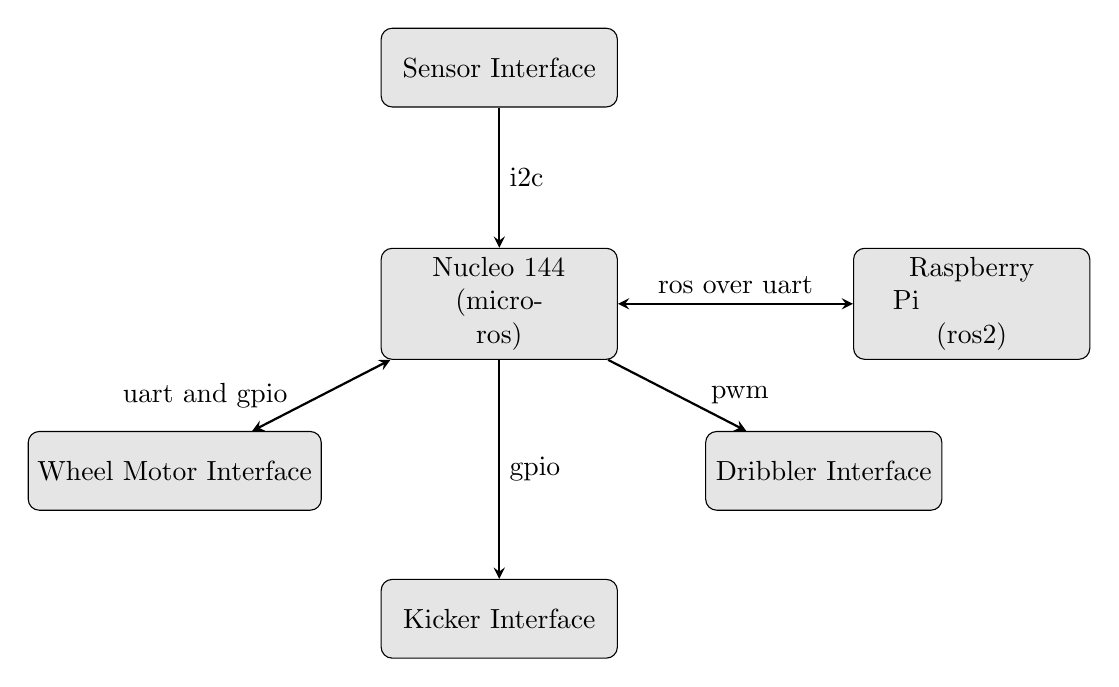
\begin{tikzpicture}[node distance=3cm]

% Nodes
\node (sensors) [block] {Sensor Interface};
\node (nucleo) [block, text width=1.7cm, below of=sensors] {Nucleo 144\newline(\acs{micro-ros})};
\node (raspberry) [block, text width=2cm, right of=nucleo, xshift=3cm] {Raspberry Pi\newline(\acs{ros2})};
\node (wheel) [block, below left of=nucleo, xshift=-2cm] {Wheel Motor Interface};
\node (kicker) [block, below of=nucleo, yshift=-1cm] {Kicker Interface};
\node (dribbler) [block, below right of=nucleo, xshift=2cm] {Dribbler Interface};

% Arrows
\draw [arrow] (sensors) -- (nucleo) node[midway, right] {\acs{i2c}};
\draw [double_arrow] (nucleo) -- (raspberry) node[midway, above] {\acs{ros} over \acs{uart}};
\draw [double_arrow] (nucleo) -- (wheel) node [midway, left, xshift=-0.3cm] {\acs{uart} and \acs{gpio}};
\draw [arrow] (nucleo) -- (kicker) node[midway, right] {\acs{gpio}};
\draw [arrow] (nucleo) -- (dribbler) node[midway, right, xshift=0.3cm] {\acs{pwm}};

\end{tikzpicture}
	\caption{A high level overview of the hardware interface and its interaction with the Raspberry Pi executable.}
	\label{fig:hardware_interface_graph}
\end{figure}

% hardware-Sensors Interface
\subsubsection{Sensor Interface}
To ensure accurate input and output for the robot, multiple sensors were utilized in the hardware interface.

\textbf{\textit{Digital Proximity, Ambient Light, RGB and Gesture Sensor(APDS-9960)}}\\
The APDS-9960 sensor was chosen due to its ability to detect ambient light, proximity, RGB color, and gestures. Our focus was to utilize the proximity detection functionality to detect objects in close proximity to the sensor. The proximity function is useful for RoboCup-Robots as they require interaction with the surrounding environment without direct contact.

The communication was established via I2C interface. The I2C bus allows for efficient data exchange between the sensor and the microcontroller, providing a reliable means of controlling the sensor and retrieving proximity data.

The proximity function of APDS-9960 sensor emit infrared (IR) light and measuring the amount of light that reflects off objects. The reflected light intensity increases when an object enters the proximity range(10 cm) of the sensor.

To establish the communication with the microcontroller STM32 via I2C, the I2C bus uses two wires: The serial data(SDA) and the serial clock(SCL), which allow multiple devices to communicate over the same bus.

To configure the proximity functionality through I2C, we write to the sensor register to configure its operation modes, then we read from a specific registers(See data sheet of APDS-9960).

\subsubsection{IP Communication}


\subsubsection{Automatic Game Controller}


%-------------------------------------------------------------------------------
% Integration
%-------------------------------------------------------------------------------

%-------------------------------------------------------------------------------
\textbf{\textit{MicroRos)}}\\
As a microcontroller, STM32 was chosen for this project. STM32 will be configured as a Micro-ROS node, which will allow interaction with Robot operation system 2 (ROS-2) using the UART communication protocol, making it possible to send and receive ROS-2 messages.
Micro-ROS client libraries are used to successfully publish and subscribe to ROS-2 topics. The UART interface is used as a communication line between STM32 and the Raspberry Pi. UART is chosen because of its simplicity and efficiency for serial communication between embedded devices.

The Raspberry Pi will serve as the central for receiving and processing the data from the STM32, utilizing ROS 2 for higher-level processing and system integration. The Raspberry Pi will also run the Micro-ROS Agent. Which is the communication pipe line between the STM32 and the ROS-2 ecosystem. The Micro-ROS Agent will handle the topics published by the STM32 (Micro-ROS node) and forward them to the corresponding ROS 2 topics on the Raspberry Pi.

\textbf{The process for communication between STM32 and Raspberry pi:}
STM32 sends(publish) sensor data(topics) over UART using the Micro-ROS client. Then the Micro-ROS agent on the Raspberry Pi will receive these topics via the UART interface and forward them to the ROS-2.


\textbf{See Figure [Number of the figure] for deeper understanding}


%===============================================================================

\begin{comment}
In this section you should describe the scientific methods you have used and how you have approached the work itself. For each objective above, identify a method for achieving the objective. The choice of method should be justified. For example, you may have made a mathematical model, used simulations, made an implementation that you tested, or done experiments that you may have evaluated using statistical methods. In the first instance, you should describe the scientific methods you used, but it is also useful to describe how you worked on the task. The Methods section also answers why you did a certain way or why you used a certain tool. So you should not only describe the "what" but also the "why". Ask yourself: can the chosen method help me to achieve the set objectives and thus answer the research question?

Choosing the right scientific method(s) is important for you to achieve your goals \cite{researchmethodology,forskningsmetodik}, so this is a point that you should discuss with your supervisor at an early stage. Also, search the literature for good descriptions of methods, and how best to write a Methods section.
\end{comment}

%===============================================================================
